% Metódy inžinierskej práce

\documentclass[10pt,oneside,slovak,a4paper]{article}
\usepackage[slovak]{babel}
\usepackage[T1]{fontenc}
\usepackage[IL2]{fontenc} % lepšia sadzba písmena Ľ než v T1
\usepackage[utf8]{inputenc}
\usepackage{graphicx}
\usepackage{amsmath}
\usepackage{url} % príkaz \url na formátovanie URL
\usepackage{hyperref} % odkazy v texte budú aktívne (pri niektorých triedach dokumentov spôsobuje posun textu)

\usepackage{cite}
\usepackage{times}



\title{Umelá inteligencia v autonómnych vozidlách\thanks{Semestrálny projekt v predmete Metódy inžinierskej práce, ak. rok 2022/23, vedenie: Matúš Koleják}} % meno a priezvisko vyučujúceho na cvičeniach

\author{Matúš Koleják\\[2pt]
	{\small Slovenská technická univerzita v Bratislave}\\
	{\small Fakulta informatiky a informačných technológií}\\
	{\small \texttt{xkolejak@stuba.sk}}
	}

\date{\small 18. november 2022} % upravte



\begin{document}

\maketitle

\begin{abstract}
Cieľom článku je zamerať sa nad potenciálnym ovplyvnením automobilovej premávky pomocou AI. S tým ako sa my, ako spoločnosť vyvíjame a napredujeme, prichádza aj otázka ako to robiť rýchlejšie, efektívnejšie poprípade bezpečnejšie. Zdravím sa život začína a aj konči. A práve to je sektor v ktorom nám môže AI pomôcť. Primárnym cieľom AI v cestnej premávke nie je život zjednodušiť, ale ho ochrániť pred potenciálnou hrozbou. AI je ako malé dieťa, učí sa. To znamená, že robí chyby. A presne to je na AI najdôležitejšie, robiť chyby s cieľom zdokonaliť sa.
\end{abstract}

%\input{novy.txt}
\newpage

\section{Výhody a nevyhody}\label{rizika}

Autonómne vozidla nám ponúkajú príležitosť využiť výhody najnovších senzorických technológií a zároveň aj umelej inteligencie. Práve táto umelá inteligencia má rozhodovať o riadení vozidla. A tým zmierniť počet rizík spájaných s cestnou premávkou. \par Pri zameraní na AI riadenie sa dostávame ku dvom protichodným smerom. Rozhodovanie medzi rizikom a výhodou technológie. Kombinácia senzorov a inteligentných technológií, poskytuje topografickú reprezentáciu cestnej premávky. Táto technológia s pomocou AI dokáže robiť bezprostrednejšie a presnejšie rozhodnutia o jazde. Vďaka AI sme taktiež schopný odstrániť problémy spojené s ľudskými slabosťami. Ako napríklad únava, intoxikácia, nesprávne vnímanie spolu s problematickými rozhodnutiami, ktoré ľudia počas jazdy robia.\par Všetky tieto fakty predstavujú bezpečnostný argument, ktorý potvrdzuje prínos pre spoločnosť. Netreba ale zabúdať na alternatívnu perspektívu, ktorá zdôrazňuje potenciál pre nové riziká.
\cite{floridi2018ai4people,doi:10.1080/08839514.2019.1600301}

%\begin{figure*}[!h]
%\centering
%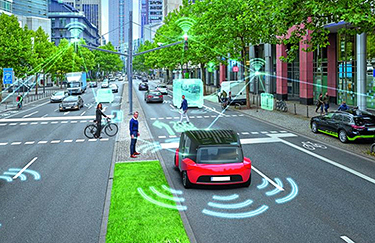
\includegraphics[scale=0.6]{viditelnost.jpg}
%\end{figure*}


\section{AKO SYSTÉM AI VNÍMA PROSTREDIE}\label{viditelnot}


\par Autonómne vozidlo získava znalosti o svojom okolí v dvoch fázach. Prvá fáza pozostáva zo skenovania vozovky pred vami s cieľom zistiť možné zmeny jazdných podmienok (okrem iného semafory a značky, prechod pre chodcov a aj závory).\cite{s19030648} 
\\~\\
Druhá fáza sa týka vnímania iných vozidiel.\ref{fig:senzory}
\par Táto časť predstavuje najreprezentatívnejšie senzory, ktoré tvoria systémy vnímania AV: ultrazvuk, RADAR, LiDAR, kamery, IMU, GNSS a RTK. Tieto senzory si môžeme prezentovať aj z pohľadu elektromagnetického spektra, ktoré aktívne alebo pasívne používa na svoju činnosť. Táto činnosť umožní získať hlbšie poznatky o výhodách a nevýhodách týchto senzorov, najmä v zhoršenom prostredí alebo v nepriaznivých poveternostných podmienkach. Na obrázku 2 je elektromagnetické spektrum je rozdelené na dve stupnice: vlnové dĺžky a frekvencie. \cite{s19030648 }

\begin{figure*}[!h]
\centering
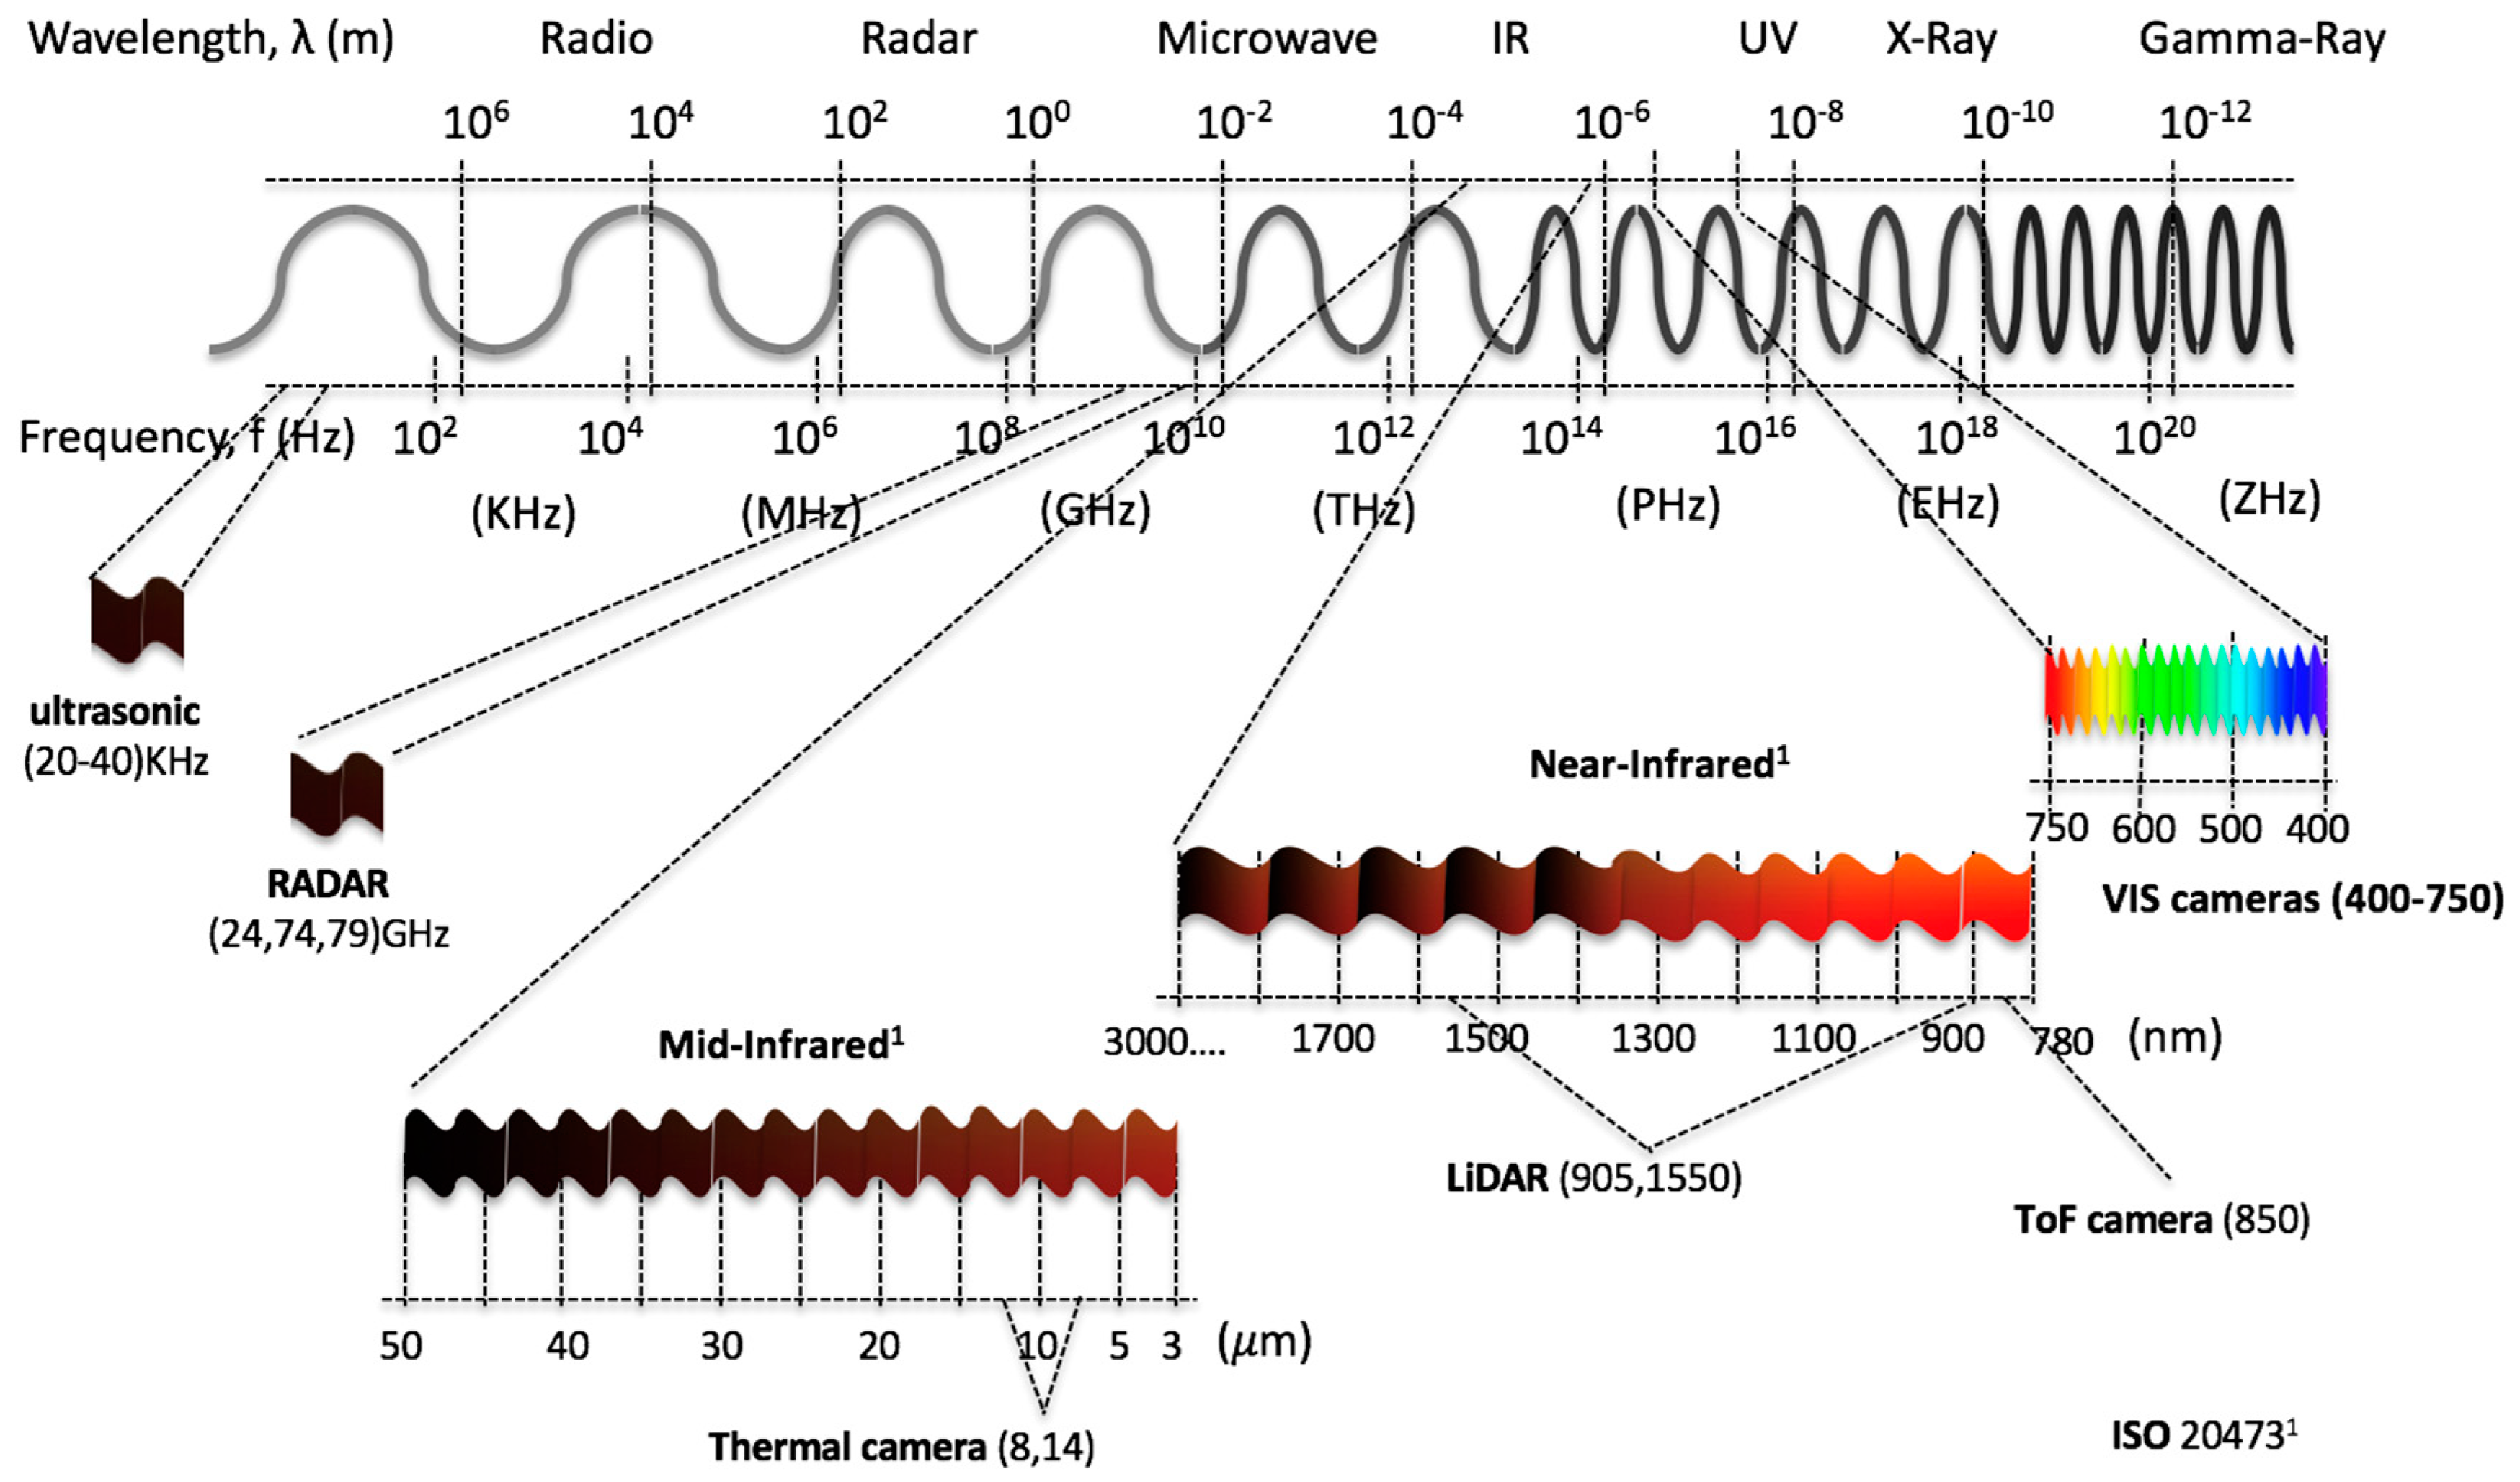
\includegraphics[scale=0.7]{senzory.png}
\label{fig:senzory}
\end{figure*}


\newpage
\subsection{Ultrazvukový senzor}\label{viditelnot}

Ultrazvukové senzory sa využívajú na meranie vzdialenosti k objektu, vďaka zvukovým vlnám v rozsahu 20 kHz až 40 kHz, ktoré sú generované magnetorezistentnou membránou. Princíp činnosti je založený na meraní doby letu zvukovej vlny(ToF) od jej vyžarovania až do prijatia ozveny:\ref{eq1}

\begin{equation} \label{eq1}
	\begin{split}
	d & = \frac{c}{2} * {ToF}
	\end{split}
	\end{equation}

\begin{center}
\centering
{
\emph{Rýchlosť c vlny je v metroch za sekundu a ToF je čas letu v sekundách.\cite{s19030648}.}
\\~\\
}
\end{center}


Tieto snímače sa vo vozidlách používajú v parkovacích systémoch, alebo ako snímače na meranie krátkej vzdialenosti pri nízkych rýchlostiach\ref{fig:ultrazvuk}. Výhoda týchto snímačov je, že sú lacné a zároveň poskytujú dobré výsledky. Napríklad vzhľadom od nepriaznivych podmienok sú nezávisle.

\begin{figure*}[!h]
\centering
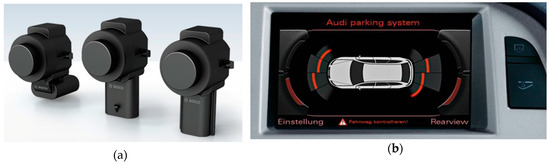
\includegraphics[scale=0.7]{senzory1.jpg}
\label{fig:ultrazvuk}
\end{figure*}

\begin{center}
\centering
{
\emph{( a )Ultrazvukové snímače do auta od firmy Bosch; b ) asistenčný parkovací systém od Audi\cite{s19030648}.}
}
\end{center}

\newpage

\subsection{Radar}
Radarové systémy pracujú vo vlnových dĺžkach rádovo v milimetroch; tieto údaje sa potom využívajú v širokej škále vojenských a civilných systémoch. Vznik inteligentných vozidiel a potreba zvýšenia bezpečnosti na cestách vyvolali používanie tohto typu zariadení v automobilovom sektore. \par Radarové systémy pre inteligentné vozidlá pracujú na frekvenciách 24/77/79 GHz, známych ako radar s milimetrovými vlnami (MMW). Radar meria vzdialenosť medzi vysielačom a objektom, výpočtom doby letu vysielaného signálu a prijatej ozveny. Radary umožňujú nielen detekciu vzdialenosti k niekoľkým cieľom, ale sú schopné presne dodať aj smer a rýchlosť cieľov.\ref{fig:radar}
\\~\\
Prijame využitie je napríklad pri detekcii mŕtveho uhlu, pri asistentovi zmeny jazdného pruhu alebo aj pri upozornení na križujúcu premávku. Vďaka týmto faktom dokáže radar výrazne zlepšiť bezpečnosť vozidla.\cite{s19030648}

\begin{figure*}[!h]

\centering
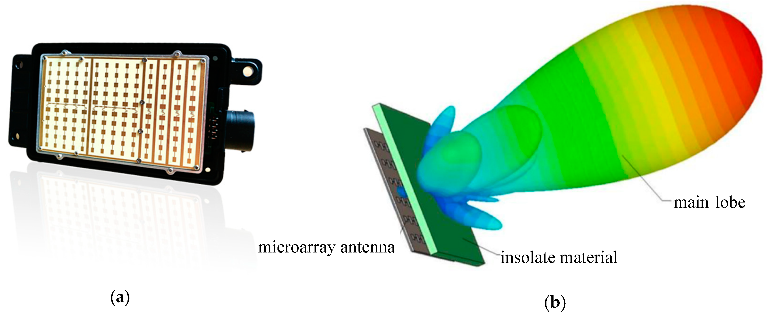
\includegraphics[scale=1]{radar.png}
\label{fig:radar}
\end{figure*}

\begin{center}
\centering
{
\emph{ a) radarová anténa Microarray; b) viaclalokový systém\cite{s19030648}.}
}
\end{center}



\subsection{Lidar (detekcia a meranie svetla)}
Systémy LiDAR fungujú na princípe: začiatok merania letu pulzného svetla (ktoré vyžaruje laserová dióda), až po dobu kedy je prijate žiaričom. Systémy môžu byť klasifikované podľa typu informácie ktorú získavajú (2D alebo 3D LiDAR).\cite{s19030648}

\begin{itemize}
\item 2D LiDAR získava informácie z prostredia premietaním jediného laserového lúča na rotujúce zrkadlo kolmé na os rotácie.\ref{fig:lidar}

\item 3D LiDAR umožňuje získať 3D mapu prostredia s veľkou presnosťou; na tento účel používajú sadu diódových laserov namontovaných na podstavci, ktorý sa otáča vysokou rýchlosťou.\ref{fig:lidar}
\end{itemize}

\newpage

\begin{figure*}[!h]
\centering
\includegraphics[scale=0.8]{lidar.jpg}

\label{fig:lidar}
\end{figure*}

\begin{center}
\centering
{
\emph{Prevádzkové schémy: (a) Rotujúci 2D LiDAR, (b) Rotujúci 3D LiDAR, 
(c)polovodičový 3D LiDAR\cite{s19030648}.}
}
\end{center}


\subsection{Kamery}
V systéme vnímania autonómnych vozidiel a z hľadiska vlnovej dĺžky prijímanej zariadením možno kamery klasifikovať ako viditeľné (VIS) alebo infračervené (IR). \cite{s19030648}

\begin{itemize}
\item Kamery VIS zachytávajú vlnové dĺžky medzi 400 nm až 780 nm \ref{fig:tabulka}, rovnako ako ľudské oko. \par Viditeľné spektrum je rozdelené do troch pásiem alebo kanálov: R, G a B, ktoré budú kódované oddelene. Tieto zariadenia sa najčastejšie používajú v systémoch AV vnímania na získavanie informácií o okolí vozidla vďaka ich nízkej cene, vysokej kvalite informácií o farbách a vysokému rozlíšeniu. Obrovský objem dát generovaných pomocou zariadenia predpokladá ďalší problém pre systém spracovania.

\item Kamery sú pasívne senzory, ktoré pracujú v infračervených (IR) vlnových dĺžkach medzi 780 nm až 1 mm.\par Existuje mnoho zariadení, ktoré pracujú v tomto spektre, pretože existuje menej svetelných interferencií (napr. LiDAR). Systémy vnímania, ktoré zahŕňajú IR kamery\cite{gade2014thermal,olmeda2011far}  pracujú v oblasti blízkej infračervenej oblasti (NIR: 780 nm–3 mm) alebo strednej infračervenej oblasti (MIR: 3 mm–50 mm, známe ako termokamery). Použitie NIR zvyčajne nahrádza alebo dopĺňa kamery VIS. IR kamery sa používajú: (1) V situáciách, kde sú špičky osvetlenia; napríklad pri výjazde z tunela, pri jazde pred slnkom alebo keď auto pretína dlhé svetlo; a pri detekcii horúceho tela, ako sú chodci. \cite{gonzalez2016pedestrian,sun2011night,john2015pedestrian}
\end{itemize}

\newpage

\begin{figure*}[!h]
\centering
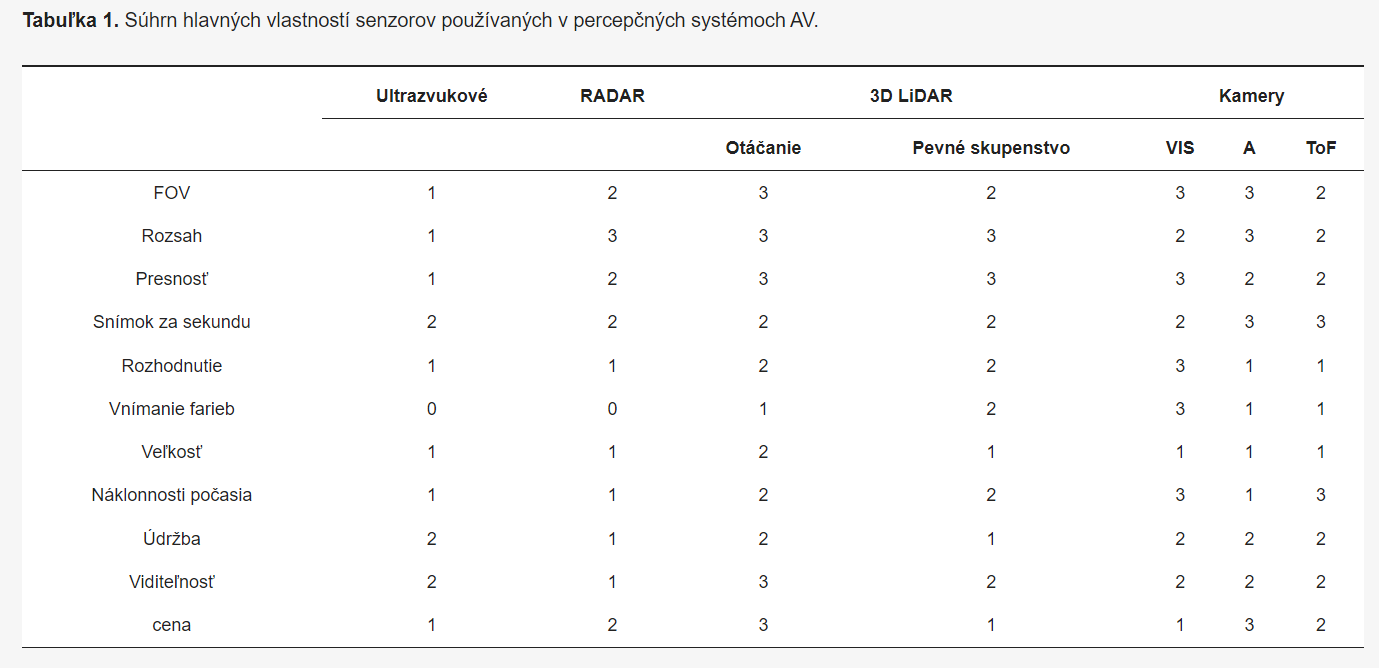
\includegraphics[scale=0.5]{tabulka.png}
\label{fig:tabulka}
\end{figure*}

\begin{center}
\centering{
\emph{ \ref{fig:tabulka} Tabuľka zobrazuje súhrn výhod a nevýhod senzorov analyzovaných v tejto časti. V tabuľke je zobrazených 11 znakov, ktoré boli kvantifikované v súlade s údajmi získanými v tomto prehľade. Kvantifikácia bola vykonaná pomocou štyroch skóre na zjednodušenie procesu: 0 – žiadne, 1 – nízke, 2 – stredné a 3 – vysoké. Prvých šesť funkcií predstavuje maximálnu kvalitu s najvyšším skóre a zvyšok získal najlepšiu kvalitu s minimálnym skóre\cite{s19030648}.}}
\end{center}


\section{Ciele}
Umelá inteligencia v Autonómnych vozidlách sa rozhoduje podľa dvoch koncepčných rámcov týkajúcich sa rozhodovacej kapacity a zmierňovania rizika\ref{rizika}. Aj keď prichádza mnoho naliehavých otázok týkajúcich sa toho, ako najlepšie skúmať a predvídať spoločenský dopad vznikajúcich technológií z hľadiska rizika \cite{asveld2009ethics}, nápadne málo pozornosti sa venuje koncepčným analýzam \cite{asveld2009ethics}. \par Tieto koncepčné analýzy zdôrazňujú nielen nedostatky vo vyšetrovaní technologických rizík a morálky, ale aj zjavnú medzeru v analytických metódach, ktoré riešia vznikajúci fenomén technologických rizík. Je tu nevyhnutná potreba zvýšenia vzdelania, aby sa umožnilo rôznorodému množstvu zainteresovaných strán prispievať k problémom súvisiacim so spoločenským využívaním technológií AI. Čo sa týka bezpečnosti AI tak tu taktiež vzniká nový etický problém. Napríklad v prípade, v ktorom by AI mala rozhodovať o živote a smrti.
~\cite{doi:10.1080/08839514.2019.1600301,7368032}



%\begin{figure*}[tbh]
%\centering
%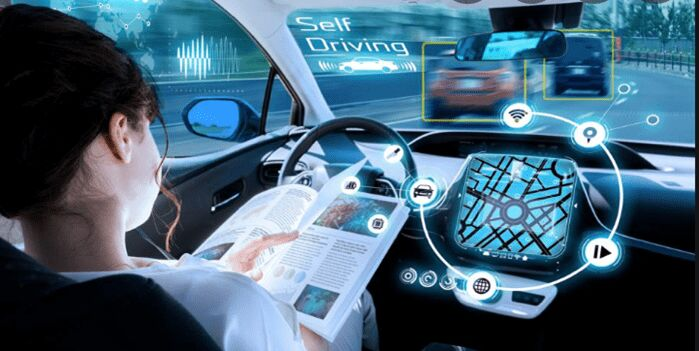
\includegraphics[scale=1.1]{auto.jpg}
%\end{figure*}
























%\acknowledgement{Ak niekomu chcete poďakovať\ldots}


% týmto sa generuje zoznam literatúry z obsahu súboru literatura.bib podľa toho, na čo sa v článku odkazujete
\bibliography{kolejakbib}
\bibliographystyle{plain} % prípadne alpha, abbrv alebo hociktorý iný
\end{document}
